
\chapter{Topology and Approximation}\label{chap3}

Since\pageoriginale we know that intersection and union of two polyhedra is a polyhedron, we may define a topology on a polyhedron $X$, by describing sets of the form $X-Y$, for $Y$ a subpolyhedron, as a basis of open sets. If, one the other hand, $X$ is a polyhedron in a finite dimensional real vector space $V$, then $V$ has various Euclidean metrics (all topologically equivalent) and $X$ inherits a metric topology. 

\begin{ex*}
These topologies on $X$ are equal.
\end{ex*}

The reason is that any point of $V$ is contained in an arbitrary small open cell, of the same dimension as $V$.

It is easy to see tht a closed simplex with this topology is compact. Hence every polyhedron, being a finite union of simplexes is compact. The graph of a polyhedral map is then compact, and hence $f$ is continuous. Thus we have an embedding of the category of polyhedra and polyhedral maps into the category of compact metric spaces and continuous maps.

It is with respect to any metric giving this topology that our approximation theorems are phrased.

A polyhedron is an absolute neighbourhood retract, and the results that we have are simply obtained from a hard look at such results for A.N.R's.

It turns our that we obtain a version of the simplicial approximation\pageoriginale theorem, which was the starting point, one may say, of the algebraic topology of the higher dimensional objects. The theorem has been given a `relative form' by Zeeman, and we shall explain a method which will give this as well as other related results.

We must first say something about polyhedral neighbourhoods.

\section{Neighbourhoods that retract}\label{chap3-sec3.1}

Let $\mathscr{P}\subset \mathcal{Q}$ be regular presentations. Consider the open cells $C$ of $\mathcal{Q}$, with $\overline{C}\cap |\mathscr{P}|\neq \emptyset$, together with $A$, $A<C$, $A\in \mathcal{Q}$, for such $C$. The set of all these open cells is a subpresentations $\mathscr{N}$ of $\mathcal{Q}$. $|\mathscr{N}|$ is a neighbourhood of $|\mathscr{P}|$ in $|\mathcal{Q}|$. For, if $\mathscr{N}'$ is the set of cells $C'\in \mathcal{Q}$ such that $\overline{C}'\cap |\mathscr{P}|=\emptyset$, then $\mathscr{N}'$ is a subpesentation of $\mathcal{Q}$ and $|\mathcal{Q}|-|\mathscr{N}'|\subset |\mathscr{N}|$. If $\mathcal{Q}$ is simplicial, $\mathscr{N}$ can be described as the subpresentation, consisting of open simplexes of $\mathcal{Q}$ with some vertices in $\mathscr{P}$ together with their faces. 

If $\mathscr{P}\subset \mathcal{Q}$ is a subpresentation, we say that $\mathscr{P}$ is full in $\mathcal{Q}$; if for every $C\in\mathcal{Q}$ either $\overline{C}\cap |\mathscr{P}|=\emptyset$ or there is a $A\in \mathscr{P}$ with $\overline{C}\cap |\mathscr{P}|=\overline{A}$.

In the case of simplicial presentations, this is the same as saying that if an open simplex $\sigma$ of $\mathcal{Q}$ has all its vertices in $\mathscr{P}$, then $\sigma$ itself is in $\mathscr{P}$.

An example of a nonfull subpresentation:
\begin{figure}[H]
\centering
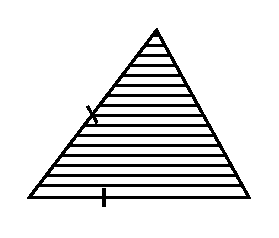
\includegraphics{figure/fig8.eps}
\end{figure}

\subsection{}\label{chap3-sec3.1.1}
If\pageoriginale $\mathscr{P}\subset \mathcal{Q}$ are regular presentations, then $d\mathscr{P}$ is full in $d\mathcal{Q}$.

For, if $\eta$ is any centering, then an element (an open simplex) of $d\mathcal{Q}$ is of the form $0(\eta(C_{0})),\ldots,\eta(C_{k}))$, $C_{k}\in\mathcal{Q}$, $C_{0}<\ldots<C_{k}$. If $C_{\ell}$, $0\leq \ell\leq k$, is the last element of the $C_{i}$'s that is in $\mathscr{P}$, then $C_{j}$, $j\leq \ell$, are necessarily in $\mathscr{P}$. Then $0(\eta(C_{0}),\ldots,\eta(C_{\ell}))\in d\mathscr{P}$, and $\overline{0}(\eta(C_{0}),\ldots,\eta(C_{k}))\cap |d\mathscr{P}|=\overline{0}(\eta(C_{0}),\ldots,\eta(C_{\ell}))$.

\setcounter{proposition}{1}
\begin{definition}\label{chap3-defi3.1.2}
If $\mathscr{P}$ is full in $\mathcal{Q}$, the {\em simplicial neighbourhood of $\mathscr{P}$ in $\mathcal{Q}$}, is the subpresentation of $d\mathcal{Q}$ consisting of all simplexes of $d\mathcal{Q}$ whose vertices $\eta(C)$ are centers of cells $C$ of $\mathcal{Q}$ with $\overline{C}\cap |\mathscr{P}|\neq \emptyset$. It is denoted by $N_{\mathcal{Q}}(\mathscr{P})$ (or $N_{\mathcal{Q}}(\mathscr{P},\eta)$ when we want to make explicit the centering).
\end{definition}

Clearly $N_{\mathcal{Q}}(\mathscr{P})$ is a full subpresentation of $d\mathcal{Q}$. It can be also described as the set of elements $\sigma$ of $d\mathcal{Q}$, for which $\overline{\sigma}\cap |d\mathscr{P}|=\overline{\sigma}\cap |\mathscr{P}|=\emptyset$ plus the faces of such $\sigma$. Hence $|N_{\mathcal{Q}}(\mathscr{P})|$ is a neighbourhood of $|\mathscr{P}|$ in the topological sense.

Such a neighbourhood as $|N_{\mathcal{Q}}(\mathscr{P})|$ of $|\mathscr{P}|$ is usually referred to as a `{\em second derived neighbourhood}' of $|\mathscr{P}|$ in $|\mathcal{Q}|$, for the following reason: If $X\subset Y$ are polyhedra; to get such a neighbourhood we first start with a regular presentation $\mathfrak{a}$ of $Y$ containing a subpresentation $\mathscr{B}$ covering $X$, derive once so that $d\mathscr{B}$ is full in $d\mathfrak{a}$, then derive again and take $|N_{d\mathfrak{a}}(d\mathscr{B})|$. 

Now we can define a simplicial map $r:N_{\mathcal{Q}}(\mathscr{P})\to d\mathscr{P}$, using\pageoriginale the property of fullness of $\mathscr{P}$ in $\mathcal{Q}$. If $C\in\mathcal{Q}$, with $\overline{C}\cap |\mathscr{P}|\neq\emptyset$, we know that there is a $A\in\mathscr{P}$, such that $\overline{C}\cap |\mathscr{P}|=\overline{A}$, and this $A$ is uniquely determined by $C$. We define $r(\eta C)=\eta A$.

\begin{ex}\label{chap3-ex3.1.3}
The map $r$ thus defined is a simplicial retraction of $N_{\mathcal{Q}}(\mathscr{P})$ onto $d\mathscr{P}$.
\end{ex}

That is $r$ is a simplicial map from $N_{\mathcal{Q}}(\mathscr{P})$ to $d\mathscr{P}$, which when restricted to $d\mathscr{P}$ is identity. $r$ defines therefore a polyhedral map, which also we shall call $r:|N_{\mathcal{Q}}(\mathscr{P})|\to |d\mathscr{P}|$. We have proved  

\setcounter{subsection}{3}
\subsection{}\label{chap3-sec3.1.4}
If $X$ is a subpolyhedron of $Y$, there is a polyhedron $N$ which is a neighbourhood of $X$ in $Y$, and there is a polyhedral retraction $r:N\to X$. 

\section{Approximation Theorem}\label{chap3-sec3.2}

We imagine our polyhedra to be embedded in real vector spaces (we have been dealing only with euclidean polyhedra) with euclidean metrics. Let $X$, $Y$ be two polyhedra, $\rho$, $\rho'$ be metrics on $X$ and $Y$ respectively coming from the vector spaces in which they are situated. If $\alpha$, $\beta:Y\to X$ are two functions, we define
$$
\rho(\alpha,\beta)={\displaystyle\mathop{\Sup}_{x\in Y}}\,\rho(\alpha(x),\beta(x))
$$

If $A$ is a subset of $X$, we define $\diam A=\sup\limits_{x,y\in A}\rho(x,y)$,
and if $B$ is a subset of $Y$, we define $\diam B={\displaystyle\mathop{\Sup}_{x,y\in B}}\,\rho'(x,y)$. 


We\pageoriginale can consider $X$ to be contained in a convex polyhedron $Q$. If $X$ is situated in the vector space $V$, we can take $Q$ to be large cube or the convex hull of $X$. Let $N$ be a second derived neighbourhood of $X$ in $Q$ and $r:N\to X$ be the retraction. Now $Q$ being convex and $N$ a neighbourhood of $X$ and $Q$, for any sufficiently small subset $S$ of $X$, $K(S)\subset N$ (recall that $K(S)$ denotes the convex hull of $S$). This can be made precise in terms of the metric; and is a uniform property since $X$ is compact. Next observe that we can obtain polyhedral presentations $\mathscr{P}$ of $X$, such that diameter of each element of $\mathscr{P}$ is less than a prescribed positive number. This follows for example from refinement process. Now theorem
is 

\begin{theorem}\label{chap3-thm3.2.1}
Given a polyhedron $X$, for every $\epsilon>0$, there exists a $\delta>0$ such that for any pair of polyhedra $Z\subset Y$, and any pair of functions $f:Y\to X$, $g:Z\to X$ with $f$ continuous and $g$ polyhedral, if $\rho(f|Z,g)<\delta$, then there exists a $\overline{g}:Y\to X$, $\overline{g}$ polyhedral, $\overline{g}|Z=g$, and $\rho(f,\overline{g})<\epsilon$.
\end{theorem}

\begin{proof}
We embed $X$ in a convex polyhedron $Q$, in which there is a polyhedral neighbourhood $N$ and a polyhedral retraction $r:N\to X$ as above. It is clear from the earlier discussion, that given $\epsilon>0$, there is a $\eta>0$, such that if a set $A\subset X$ has diameter $<\eta$, then $K(A)\subset N$ and diamter $r(K(A))<\epsilon$. Define $\delta=\eta/3$.


Now because of the uniform continuity of $f$, ($Y$ is compact), there is a $\theta>0$, such that if $B\subset Y$ and diam. $(B)<\theta$, then\pageoriginale $\diam f(B)<\delta$.

From this it follows that, still assuming $B\subset Y$, and diameter $B<\theta$, and additionally that $\rho(f|Z,g)<\delta$; that the set $f(B)\cup g(B\cap Z)$ has diameter less than $3\delta=\eta$. And hence we know that 
\begin{equation*}
\begin{cases}
K(f(B)\cup g(B\cap Z))\subset N,\quad\text{and}\\
\diam r(K(f(B)\cup g(B\cap Z)))<\epsilon.
\end{cases}\tag{*}
\end{equation*}

Then we find a presentation $\mathscr{S}$ of $Y$, such that the closure of every element of $\mathscr{S}$ has diameter less than $\theta$. Also there is a presentation $\mathscr{Z}$ of $Z$ on the closure of every element of which $g$ is linear. Refining $\mathscr{S}\cup \mathscr{Z}$ and taking derived subdivisions (still calling the presentations covering $Y$ and $Z$, as $\mathscr{S}$ and $\mathscr{Z}$ respectively), we have the following situation:

$\mathscr{Z}\subset \mathscr{S}$, are simplicial presentations of $Z\subset Y$, on each closed $\mathscr{Z}$-simplex $g$ is linear, the diameter of each closed $\mathscr{S}$-simplex $<\theta$.

We now define $h:Y\to Q$ as follows: On a $0$-simplex $v$ of $\mathscr{Z}$, $h(v)=g(v)$. On a $0$-simplex $w$ of $\mathscr{S}-\mathscr{Z}$, $h(w)=f(w)$. Extend $h$ linearly on each simplex, this is possible since $Q$ is convex. But now, if $\overline{\sigma}=[v_{0},\ldots,v_{n}]$ is the closure of a $\mathscr{S}$-simplex, then $h(\overline{\sigma})\subset K(f(\overline{\sigma})\cup g(\overline{\sigma}\cap Z))\subset N$; this is a computation made above (*) since diam. $\overline{\sigma}<\theta$.

And so $h(Y)\subset N$. Also it is the case that $h$ is polyhedral, since $h$ is liner on the closure of each simplex of $\mathscr{S}$, and on $|\mathscr{Z}|=Z$, clearly, $h$ agrees with $g$.

Define, $\overline{g}:Y\to X$ to be $r\circ h$. Since $r$ and $h$ are polyhedral\pageoriginale so is $\overline{g}$; since $h|Z=g$ and $r$ is identity on $X$; it follows that $\overline{g}|Z=g$. To compute $\rho(\overline{g},f)$ we observe that any $y\in Y$ is contained in some closed simplex $\overline{\sigma}$, $\sigma\in \mathscr{S}$, and both $f(y)$ and $h(y)$ are contained in $K(f(\overline{\sigma})\cup g(\overline{\sigma}\cap Z))$; and hence both $f(y)$ and $g(y)$ are contained in 
$$
r(K(f(\overline{\sigma})\cup g(\overline{\sigma}\cap Z)))
$$

This set by (*) has diameter $<\epsilon$. Hence $\rho(\overline{g},f)<\epsilon$.
\end{proof}

We now remark a number of corollaries:

\begin{corollary}\label{chap3-coro3.2.2}
Let $X$, $Y$, $Z$ be polyhedra, $Z\subset Y$, and $f:Y\to X$ a continuous map such that $f|Z$ is a polyhedral. Then $f$ can be approximated arbitrarily closely by polyhedral maps $g:Y\to X$ such that $g|Z=f|Z$.
\end{corollary}

The next is not a corollary of \ref{chap3-thm3.2.1}, (it could be) but follows from the discussion there.

\setcounter{subsection}{2}
\subsection{}\label{chap3-sec3.2.3}
Any two continuous maps $f_{1}$, $f_{2}:Y\to X$, if they are sufficiently close are homotopic. (Also how close depends only on $X$, not $Y$ or the maps involved). If $f_{1}$ and $f_{2}$ are polyhedral, we can assume the homotopy also to be polyhedral, and fixed on any sub-polyhedron on which $f_{1}$ and $f_{2}$ agree.

\begin{proof}
Let $N$ and $X$ be as before. Let $\eta$ be a number such that if $A\subset X$, $\diam A<\eta$, then $K(A)\subset N$. If $\rho(f_{1},f_{2})<\eta$, then $F(y,t)=tf_{1}(y)+(1-t)f_{2}(y)\in N$, for $0\leq t\leq 1$ and all $y\in Y$ and $r\cdot F$, where $r:N\to X$ is the retraction, gives the required homotopy. If $f_{1}$, $f_{2}$ are polyhedral, we can apply \ref{chap3-thm3.2.1} to obtain a polyhedral homotopy with the desired properties.
\end{proof}

\begin{remark*}
The\pageoriginale above homotopies are small in the sense, that the image of $x$ is not moved too far from $f_{1}(x)$ and $f_{2}(x)$.
\end{remark*}

\subsection{}\label{chap3-sec3.2.4}
Homotopy groups and singular homology groups of a polyhedron can be defined in terms of continuous functions or polyhedral maps from closed simplexes into $X$. The two definitions are naturally isomorphic. The same is true for relative homotopy groups, triad homotopy groups etc.

The corollary \ref{chap3-coro3.2.2} is Zemman's version of the relative simplicial approximation theorem. From this (coupled with \ref{chap4-prop4.2.13}) one can deduce (see M.\@ Hirsch, ``A proof of the nonretractibility of a cell onto its boundary'', Proc.\@ of A.M.S., 1936, Vol.\@ 14), Brouwer's theorems on the noncontractibility of the $n$-sphere, fixed point property of the $n$-cell, etc. It should be remarked that the first major use of the idea of simplicial approximation was done by L.E.J.\@ Brouwer himself; using this he defined degree of a map, proved its homotopy invariance, and incidentally derived the fixed point theorem.

It should be remarked that relative versions of \ref{chap3-thm3.2.1} are possible. For example define a pair $(X_{1},X_{2})$ to be a space (or a polyhedron) and a subspace (or a subpolyhedron) and continuous (or polyhedral) maps $f:(X_{1},X_{2})\to (Y_{1},Y_{2})$ to be the appropriate sort of function $X_{1}\to X_{2}$ which maps $X_{2}$ into $Y_{2}$. Then Theorem \ref{chap3-thm3.2.1} can be stated in terms of pairs and the proof of this exactly the same utilising modifications of \ref{chap3-sec3.1.4} and the remarks at the beginning of \ref{chap3-sec3.2} which are valid for pairs.

Another relative version of interset is the notion of {\em polyhedron\pageoriginale over $A$}, that is, a polyhedral map $\mathcal{L}:X\to A$. A map $f:(\alpha:X\to A)\to (\beta:Y\to A)$ is a function $f:X\to Y$ such that $\alpha=\beta\cdot f$; we can consider either polyhedral or continuous maps. The reader should state and prove \ref{chap3-thm3.2.1} in this context (if possible).

\section{Mazur's criterion}\label{chap3-sec3.3}

We shall mention another result (see B.\@ Mazur ``The definition of equivalence of combinatorial imbeddings'' Publications Mathematiques, No.3, I.H.E.S., 1959) at this point, which shows that, in a certain sense, close approximations to embeddings are embeddings (in an ambient vector space).

Let $\mathscr{Z}$ be a simplicial presentation of $X$, and let $V$ be a real vector space. Let $\mathscr{Z}_{0}$ denote the set of vertices of $\mathscr{Z}$. Given a function $\varphi:\mathscr{Z}_{0}\to V$, we can define an extension $\widetilde{\varphi}:|\mathscr{Z}|\to V$ by mapping each simplex linearly. Clearly if $Y\subset V$ is any polyhedron containing $\widetilde{\varphi}(X)$, the resulting map $X\to Y$ is polyhedral. We call $\widetilde{\varphi}$ the linear extension of $\varphi$. 
$\widetilde{\varphi}$ is called an {\em embedding} if it maps distinct points of $X$ into distinct points in $V$.

\subsection{}\label{chap3-sec3.3.1}
(Mazur's criterion for non-embeddings)

If the linear extension $\widetilde{\varphi}$ of $\varphi:\mathscr{Z}_{0}\to V$ is not an embedding, then there are two open simplexes $\sigma$ and $\tau$ of $\mathscr{Z}$, with no vertices in common, such that $\widetilde{\varphi}(\sigma)\cap \widetilde{\varphi}(\tau)\neq \emptyset$. 

\begin{proof}
The proof is in two stages.
\begin{enumerate}
\renewcommand{\theenumi}{\Alph{enumi}}
\renewcommand{\labelenumi}{(\theenumi)}
\item If $\sigma=0(v_{0},\ldots,v_{n})$ and $\{\varphi(v_{0}),\ldots,\varphi(v_{n})\}$ is not independent, then there are faces $\sigma_{1}$ and $\sigma_{2}$ of $\sigma$, without\pageoriginale vertices in common, such that $\widetilde{\varphi}(\sigma_{1})\cap \widetilde{\varphi}(\sigma_{2})\neq \emptyset$ (This is just \ref{chap1-prop1.2.6}).

\item Thus we can assume that for every $\sigma$ of $\mathscr{Z}$, $\widetilde{\varphi}(\sigma)$ is also an open simplex of the same dimension. Consider pairs of distinct open simplexes $\{\rho,\rho'\}$ such tht $\widetilde{\varphi}(\rho)\cap \widetilde{\varphi}(\sigma')\neq \emptyset$. Let $\{\sigma,\tau\}$ be such a pair, which in addition has the property $\dim \sigma+\dim \tau$ is minimal among such pairs. We can now show that $\sigma$ and $\tau$ have no vertex in common. If $\sigma=0(v_{0},\ldots,v_{m})$ and $\tau=0(w_{1},\ldots,w_{n})$, then if $\widetilde{\varphi}(\sigma)\cap \widetilde{\varphi}(\tau)\neq 0$, there is an equation
$$
r_{0}\varphi(v_{0})+\cdots+r_{m}\varphi(v_{m})=s_{0}\varphi(w_{1})+\cdots+s_{n}\varphi(w_{n})
$$
with $r_{0}+\cdots+r_{m}=1=s_{0} + s_{1}\cdots+s_{n}$. Here $r_{i}$ and $s_{i}$ are strictly greater than $0$, for otherwise $\dim \sigma+\dim \tau$ will not be minimal.
\end{enumerate}

Now if and have a common vertex, say, for example, $v_{0}=w_{0}$, and $r_{0}\geq s_{0}$, we can write
$$
(r_{0}-s_{0})\varphi(v_{0})+\sum\limits_{i\geq 1}r_{i}\varphi(v_{i})=\sum\limits_{j\geq 1}s_{j}\varphi(w_{j}).
$$

Multiplying by $(1-s_{0})^{-1}$, we see that some face of $\widetilde{\varphi}(\sigma)$ intersects a proper face $\widetilde{\varphi}(0(w_{1}),\ldots,w_{n}))$ of $\widetilde{\varphi}(\sigma)$. So that $\sigma$ and $\tau$ had not the minimal dimension compatible with the properties $\sigma\neq \tau$, $\widetilde{\varphi}(\sigma)\cap \widetilde{\varphi}(\tau)\neq \emptyset$.
\end{proof}

Now it easily follows, since to check $\widetilde{\varphi}$ is an embedding we need only check that finitely many compact pairs $\{(\widetilde{\varphi}(\overline{\sigma}),\widetilde{\varphi}(\overline{\tau})),\overline{\sigma}\cap \overline{\tau}=\emptyset\}$ do not intersect;

\setcounter{proposition}{1}
\begin{proposition}\label{chap3-prop3.3.2}
Let\pageoriginale $\mathscr{Z}$ be a simplicial presentation of $X$ contained in a vector space $V$, let $\mathscr{Z}_{0}$ be the set of vertices. Then there exists an $\epsilon>0$, such that if $\varphi:\mathscr{Z}_{0}\to V$ is any function satisfying $\rho(v,\varphi(v))<\epsilon$ for all $v\in \mathscr{Z}_{0}$, then the linear extension $\widetilde{\varphi}:X\to V$ is an embedding.
\end{proposition}

This is a sort of stability theorem for embeddings, that is, if we perturb a little the vertices of an embedded polyhedron, we still have an embedding.





